%%%%%%%%%%%%%%%%%%%%%%%%%%%%%%%%%%%%%%%%%
% University Assignment Title Page 
% LaTeX Template
% Version 1.0 (27/12/12)
%
% This template has been downloaded from:
% http://www.LaTeXTemplates.com
%
% Original author:
% WikiBooks (http://en.wikibooks.org/wiki/LaTeX/Title_Creation)
%
% License:
% CC BY-NC-SA 3.0 (http://creativecommons.org/licenses/by-nc-sa/3.0/)
% 
% Instructions for using this template:
% This title page is capable of being compiled as is. This is not useful for 
% including it in another document. To do this, you have two options: 
%
% 1) Copy/paste everything between \begin{document} and \end{document} 
% starting at \begin{titlepage} and paste this into another LaTeX file where you 
% want your title page.
% OR
% 2) Remove everything outside the \begin{titlepage} and \end{titlepage} and 
% move this file to the same directory as the LaTeX file you wish to add it to. 
% Then add \input{./title_page_1.tex} to your LaTeX file where you want your
% title page.
%
%%%%%%%%%%%%%%%%%%%%%%%%%%%%%%%%%%%%%%%%%
%\title{Title page with logo}
%----------------------------------------------------------------------------------------
%	PACKAGES AND OTHER DOCUMENT CONFIGURATIONS
%----------------------------------------------------------------------------------------

\documentclass[12pt]{article}
\usepackage[english]{babel}
\usepackage[utf8x]{inputenc}
\usepackage{amsmath,amssymb,amsthm}
\usepackage{amsfonts,amsthm,xcolor,color}
\usepackage{graphicx}
\usepackage[colorinlistoftodos]{todonotes}
%\usepackage{gen_def}
%\usepackage[margins, adjustmargins]{./trackchanges-0.7.0/LatexPackage/trackchanges}
\usepackage[inline]{trackchanges}

% Setup commands for 6 editors (one more than allowed).
\addeditor{GM1}
\addeditor{GM2}
\addeditor{GM3}
\addeditor{GM4}
\addeditor{GM5}

\begin{document}

\begin{titlepage}

\newcommand{\HRule}{\rule{\linewidth}{0.5mm}} % Defines a new command for the horizontal lines, change thickness here

\newcommand{\Deriv}[3]{\dfrac{\partial^#1 #2}{\partial #3^#1}}

\center % Center everything on the page
 
%----------------------------------------------------------------------------------------
%	HEADING SECTIONS
%----------------------------------------------------------------------------------------

\textsc{\LARGE EMORY UNIVERSITY}\\[0.3cm] % Name of your university/college
\textsc{\LARGE DEPARTMENT OF MATHEMATICS  }\\[0.3cm]
\textsc{\Large Atlanta (GA) USA }\\[0.3cm]
\textsc{\Large Project}\\[0.5cm] % Major heading such as course name
 % Minor heading such as course title

%----------------------------------------------------------------------------------------
%	TITLE SECTION
%----------------------------------------------------------------------------------------

\HRule \\[0.4cm]
{ \large \bfseries MATH MODELING OF CORONAVIRUS OUTBREAK}\\[0.03cm] % Title of your document
\HRule \\[1.5cm]

 
%----------------------------------------------------------------------------------------
%	AUTHOR SECTION
%----------------------------------------------------------------------------------------

\begin{minipage}{0.4\textwidth}
\begin{flushleft} \large
\emph{Submitted By:} \\
Group  \\ % Your name
\end{flushleft}
\end{minipage}
~
\begin{minipage}{0.4\textwidth}
\begin{flushright} 
\small \emph{Authors:}\\[0.3cm]
John \textsc{Smith 1}\\[0.3cm] % Your name
John \textsc{Smith 2}\\[0.3cm] % Your name
John \textsc{Smith 3}\\[0.3cm] % Your name
John \textsc{Smith 4}\\[0.3cm] % Your name
John \textsc{Smith 5}\\[0.3cm] % Your name
\end{flushright}
\end{minipage}\\[1cm]

% If you don't want a supervisor, uncomment the two lines below and remove the section above
%----------------------------------------------------------------------------------------
%	DATE SECTION
%----------------------------------------------------------------------------------------

{\Large Spring 2020 \\Report}\\[1cm] % Date, change the \today to a set date if you want to be precise

%----------------------------------------------------------------------------------------
%	LOGO SECTION
%----------------------------------------------------------------------------------------


\includegraphics[height=2cm,width=7cm]{EU_hz_280.png}\\[1cm] % Include a department/university logo - this will require the graphicx 
 
%----------------------------------------------------------------------------------------

\vfill % Fill the rest of the page with whitespace

\end{titlepage}


\newpage
While the World is facing one of the most severe and dangerous emergencies of the last years, Mathematicians can stand aside Medical Doctors and all Healthcare professionals. Mathematics is the language of science, but also provides the tools for quantifying the evolution of the outbreak and, ultimately, predicting its effects. This is a time for Mathematicians to take action. In particular, we want Emory students to feel engaged by the task of translating their knowledge from the classroom to the society. 
In the course MATH212 (Differential Equations), you, students, learn how to describe problems with differential equations and systems of differential equations. In MATH250, you learn the foundations of mathematical thinking and advancing knowledge. In MATH351 (Partial Differential Equations), you learn how more complex problems can be described by Partial Differential Equations. In MATH315 (Numerical Analysis), they learn how to find quantitative solutions for complex problems with numerical approximations. In MATH345 (Mathematical Modeling), you learn how to gather different competences to formulate a mathematical description to real problems and, eventually, how to evaluate its results. In MATH361 and MATH362, you learn how to give a probabilistic description to problems and, possibly, quantify the impact of a lack of knowledge on the quantitative answers that we obtain from mathematical models.
All these concepts and notions may be beneficial NOW for our society under attack from this virus, together with your fresh energy, enthusiasm, creativity, a sense of purpose!
The outbreak of a disease (like Coronavirus) can be described in terms of a system of Ordinary Differential equations known as SIR (Susceptible-Infected-Recovered) and its variants. The diffusion of a population in space can be described by a Partial Differential Equation (the diffusion or heat equation). With these tools, it is possible to create a mathematical model that may
1) predict the dynamics of the outbreak and the regions of the World or the Country more exposed;
2) describe the effects of countermeasures
With numerical tools, it is possible to approximate the solution of these models and to provide decision-making support.
The task is not easy, and it requires the combination of data and models to obtain reliable predictions. We ask the students of Emory (in Math, but also Biology) to express their citizenship by using their knowledge of math, applied math, numerical analysis, physical and biological modeling to help to construct accurate and reliable predictions. 
Students can form teams (that are, however, supposed to work remotely) to join their different backgrounds - or can work individually, to provide accurate modeling following the guidelines below.
The guidelines to take this challenge are illustrated below.
The projects will be evaluated by a committee of the Department of Mathematics and …
The Department of Mathematics will award the three best projects…
Your contribution is significant. Healthcare and society need Mathematics.



\newpage
\sffamily
\pagecolor{yellow}
\pagenumbering{gobble}

\section*{Assignment}

MODELING CORONAVIRUS OUTBREAK

As China faced the terrible outbreak of Coronavirus, which is hitting Italy and Europe and probably will hit the USA in the next weeks, 
your task is to formulate and test a model for describing the dynamics of the outbreak in the USA. You should formulate a mathematical model based on the data available at the website

\begin{verbatim}
https://www.arcgis.com/apps/opsdashboard/index.html#/
bda7594740fd40299423467b48e9ecf6
\end{verbatim}

 

The ultimate purpose of your model is to predict the timeline of the outbreak in the USA.   
 Use the data available for China and Italy to assess the reliability of your model (for instance, using data in Jan and Feb to make predictions in March)
 and test the results.
The model can include a compartment subdivision to include the different States of the USA or a space dependence (PDE). 
Other options may include:
\begin{enumerate}
      \item consider the age-structure of the population (as the mortality is significantly different with the age);
      \item consider genders (as the mortality is higher in males);
      \item consider geographical features that may slow or accelerate the spreading;
      \item consider climatic effects to test the possible impact of the temperatures on the outbreak;
      \item consider the impact of non-pharmacological and pharmacological remedies (like closing schools, reducing or cancelling events, vaccines)
      \item (ADVANCED TOPIC) consider data assimilation techniques like Kalman filtering to formulate sequential predictions.
\end{enumerate}

Formulate and motivate a mathematical model, discuss its reliability as a prediction tool.
Identify the most important simplifying assumptions and possible directions for future improvements.






\newpage
\pagecolor{white}
\rmfamily
\setcounter{page}{1}
\pagenumbering{arabic}

\begin{abstract}
EXECUTIVE SUMMARY (MAX 1 PAGE)
\end{abstract}

\section{Introduction}
\newcommand{\Deriv}[3]{\dfrac{\partial^#1 #2}{\partial #3^#1}}

20 pag limit (excluding the bibliography, including the executive summary)

Your introduction goes here! 

Some examples of commonly used commands and features are listed below, to help you get started.

%If you have a question, please use the support box in the bottom right of the screen to get in touch. 

\section{Some \LaTeX{} Examples}
\label{sec:examples}

\subsection{Sections}

Use section and subsection commands to organize your document. \LaTeX{} handles all the formatting and numbering automatically. Use ref and label commands for cross-references.

\subsection{Comments}

Comments can be added to the margins of the document using the \todo{Here's a comment in the margin!} todo command, as shown in the example on the right. You can also add inline comments too:

\todo[inline, color=green!40]{This is an inline comment.}

\subsection{Tables and Figures}

Use the table and tabular commands for basic tables --- see Table~\ref{tab:widgets}, for example. You can upload a figure (JPEG, PNG or PDF) using the files menu. To include it in your document, use the includegraphics command as in the code for Figure~\ref{fig:frog} below.

% Commands to include a figure:
\begin{figure}
\centering
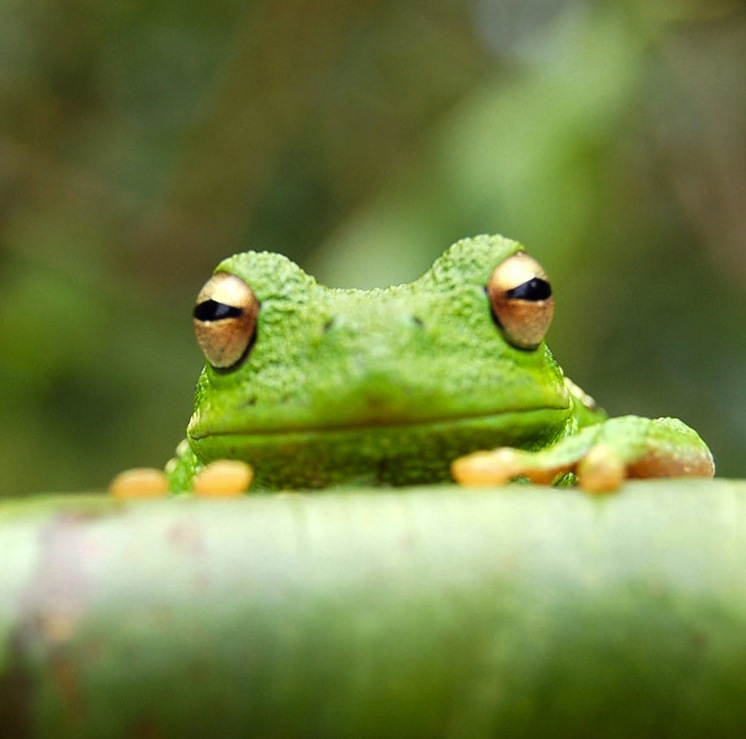
\includegraphics[width=0.5\textwidth]{frog.jpg}
\caption{\label{fig:frog}This is a figure caption.}
\end{figure}

\begin{table}
\centering
\begin{tabular}{l|r}
Item & Quantity \\\hline
Widgets & 42 \\
Gadgets & 13
\end{tabular}
\caption{\label{tab:widgets}An example table.}
\end{table}

\subsection{Mathematics}

\LaTeX{} is great at typesetting mathematics. Let $X_1, X_2, \ldots, X_n$ be a sequence of independent and identically distributed random variables with $\text{E}[X_i] = \mu$ and $\text{Var}[X_i] = \sigma^2 < \infty$, and let

\begin{equation}\label{eq:1}
S_n = \frac{X_1 + X_2 + \cdots + X_n}{n}
      = \frac{1}{n}\sum_{i}^{n} X_i
\end{equation}

This is a derivative
$$
\Deriv{2}{u}{x}
$$

denote their mean. Then as $n$ in equation \eqref{eq:1} approaches infinity, the random variables $\sqrt{n}(S_n - \mu)$ converge in distribution to a normal $\mathcal{N}(0, \sigma^2)$.

\subsection{Lists}

You can make lists with automatic numbering \dots

\begin{enumerate}
\item Like this,
\item and like this.
\end{enumerate}
\dots or bullet points \dots
\begin{itemize}
\item Like this,
\item and like this.
\end{itemize}

%We hope you find write\LaTeX\ useful, and please let us know if you have any feedback using the help menu above.

\subsection{Working with an offline trackchange}

This template includes the library {\tt trackchanges}
to perform offline trackchanges.

A list of possible editors is added at the source file line n. 46.
For now, each Group Member is denoted by GMn where n is a number.
Feel free to edit with your initials.
This will help tracking who made the comments.

Now, some examples.

This is a sentence but \add[GM1]{GM1 thinks it should be more complete}.

This is another sentence but GM2 thinks that the word \change[GM2]{sentence}{phrase} is wrong.

This a third sentence, but GM5 wants to remove the word \remove[GM5]{sentence}.  

%GM4 thinks that \add[GM4]{(this is all insane)}{ He is probably right}.

GM3 says that a reference is needed \refneeded[GM3]{}.


To do a rapid analysis of all the comments, there is a python 
script that opens a gui for processing the text and accept/reject/modify the comments.Look at the directory {\tt trackchanges-0.7.0}. 

Otherwise, you can do this manually 


\section{How to include References}

In this system, you write a file with extension bib and then you include references with
the command \texttt{cite}, \cite{gashi2019influence},
The count of pages (max. 20) does not include the References.

\newpage
\pagenumbering{gobble}
\bibliographystyle{plain}
\bibliography{References}


\end{document}